\documentclass{article}
\usepackage[margin=1in]{geometry}
\usepackage{graphicx, indentfirst, amssymb, amsmath, placeins, xurl, booktabs}
\usepackage[hidelinks,hypertexnames=false]{hyperref}

\title{Replication of ``TDA of Financial Time Series" Methodology \& Extension to Pre-COVID Setting.\\
Statistics 565 Final Report}
\author{Artem Ivaniuk}
\date{\today}

\begin{document}

\maketitle

\section*{Abstract}
This project replicates the topological data analysis framework developed by Gidea and Katz in ``Topological Data Analysis of Financial Time Series:
Landscapes of Crashes" (\url{https://arxiv.org/pdf/1703.04385}) for daily U.S. equity indices and extends the sample through 2020. For each trading date, I construct rolling windows of multivariate log-return vectors and analyze their geometric structure using persistence diagrams and persistence landscapes. I then track persistence landscape norms over time and compare them with VIX behavior during major periods of market stress.

The replication results show the clearest buildup patterns around the 2008 Lehman Brothers collapse, where persistence landscape norms and volatility measures increase together before the crisis. Results for the Dot-com period are less consistent across different statistical checks, suggesting that the relationship between topology-based indicators and financial stress may vary across events. Extending the analysis through the COVID-19 crash shows that the same framework does not generate a strong early-warning signal under the unchanged specification. Overall, the results suggest that persistence-based topological measures can provide useful information about market structure, but they are better interpreted as complementary indicators alongside traditional volatility measures rather than as stand-alone forecasting tools.

\section{Introduction}
Financial markets are usually analyzed using familiar quantities such as returns, volatility, and correlations between assets. Gidea and Katz propose a different approach by studying the geometric structure of market returns using tools from topological data analysis (TDA). Instead of focusing only on averages or pairwise relationships, their framework examines how collections of returns are organized in higher-dimensional space over time. For this project, I replicate the empirical pipeline from Gidea and Katz using daily Yahoo Finance data for four major U.S.\ equity indices: the S\&P~500, DJIA, Nasdaq Composite, and Russell~2000. Second, I extend the sample through 2020 to test whether the same methodology captures behavior around the COVID-19 market crash without changing the original parameter choices or implementation.

The central idea behind the paper is that market stress may appear not only through rising volatility, but also through changes in the overall geometric structure of joint returns, which may be impossible to observe without utilizing topology-based time series analysis. Persistent homology provides a way to summarize these geometric changes across multiple scales. By tracking persistence landscape norms (defined in section \ref{sec:methods}) through time, the paper attempts to determine whether topological summaries contain useful information before major market disruptions.

\newpage
\section{Methodology}
\label{sec:methods}

For each trading date $t$, I construct a rolling window of the previous $w$ daily log-return vectors, where $w\in\{50,100\}$. Each day in the window corresponds to a point in $\mathbb{R}^4$, using returns from the S\&P~500, DJIA, Nasdaq Composite, and Russell~2000. The resulting collection of points forms a cloud $X_t$ that represents how the four markets moved together during that time period.

To study the structure of these point clouds, I use persistent homology with a Vietoris--Rips filtration. Informally, the filtration starts by treating each point independently and then gradually connects nearby points as a scale parameter $\epsilon$ increases. When enough connections appear, loops and higher-dimensional structures can form. In this report, the main focus is on $H_1$, which tracks loop structures within the data.

Each loop is associated with a birth scale $b$ and a death scale $d$, producing persistence pairs $(b,d)$. Features that persist for longer periods, measured by $d-b$, are interpreted as more stable geometric structures, while short-lived features are usually treated as noise. These persistence pairs are summarized using persistence landscapes, which convert the persistence diagram into a collection of functions $\lambda_k(x)$. This allows the data to be analyzed using standard function-space summaries such as $L^1$ and $L^2$ norms.

Intuitively, the goal is to transform a complex four-dimensional return cloud into a simpler signal that measures whether market behavior is becoming more structured during periods of stress. If joint returns begin reorganizing before a crisis, this may appear through larger or more persistent geometric loops, leading to higher persistence landscape norms.

Data are collected from Yahoo Finance using \texttt{yfinance}. Adjusted closing prices are downloaded for the four equity indices and for VIX, which serves as a benchmark volatility measure. Daily log-returns are computed as
$r_{i,j}=\log(P_{i,j}/P_{i-1,j})$.
Persistent homology calculations are performed using \texttt{ripser}, and persistence landscapes are computed for each rolling window. 

Following the framework used in the paper and the course replication workflow, I compare persistence landscape norms with market events using rolling variance analysis, spectral analysis, and Kendall-$\tau$ trend tests over 250-trading-day windows before major crisis dates. Figure~\ref{fig:rep_data} in the appendix confirms that the aligned adjusted-close series and log-return calculations are consistent before applying the topological pipeline.

\section{Replication results}
\label{sec:results}

Figure~\ref{fig:rep_norms} shows the trajectories of the $L^1$ and $L^2$ persistence landscape norms over time. Both measures tend to increase during periods associated with higher market stress, motivating a closer look at the major crisis periods studied in the original paper.

\FloatBarrier
\begin{figure}[htbp]
    \centering
    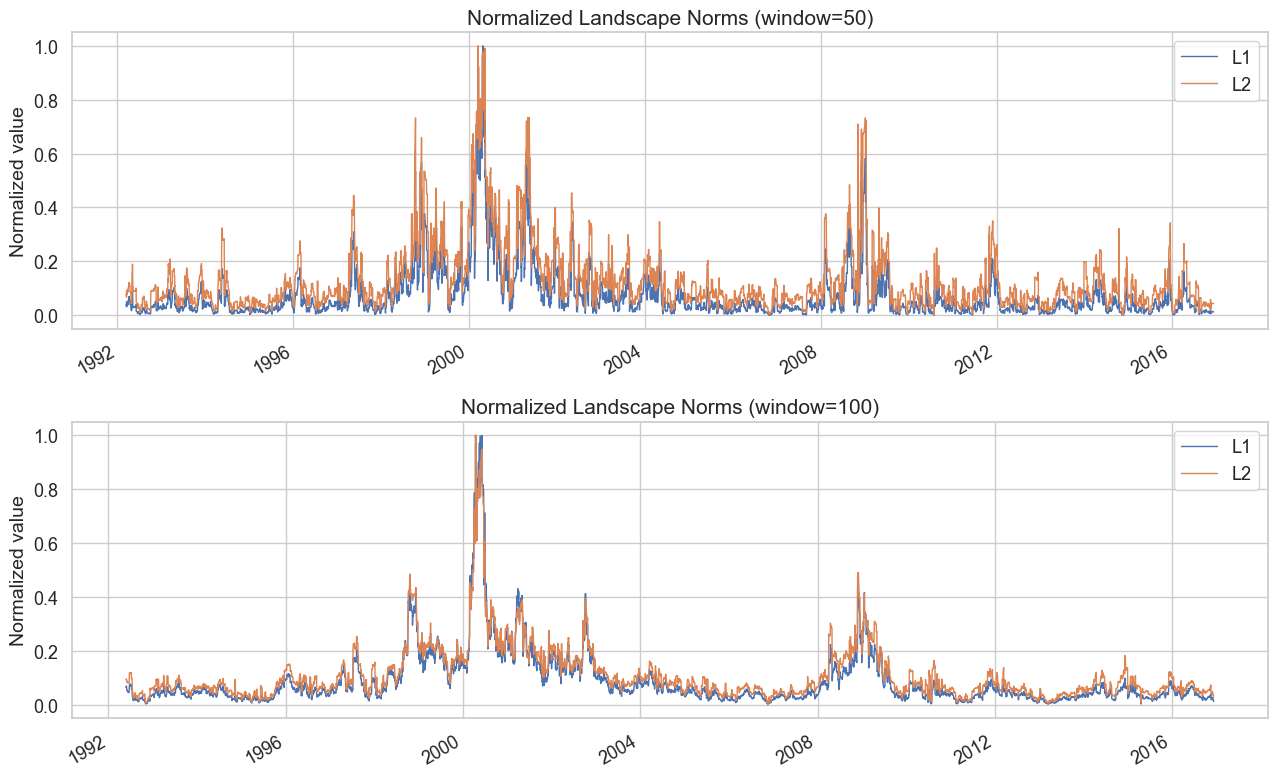
\includegraphics[width=0.7\textwidth]{figures/figure_cell13_out0.png}
    \caption{Persistence landscape norm trajectories ($L^1$, $L^2$)}
    \label{fig:rep_norms}
\end{figure}
\FloatBarrier

Figure~\ref{fig:rep_events} compares normalized aggregate equity levels, standardized $L^1$ norms for $w=50$, and normalized VIX around the Dot-com crash and the Lehman Brothers collapse. The Lehman period produces the clearest agreement between persistence landscape norms and volatility measures. Both $L^1$ and VIX rise noticeably before the main market disruption, which matches the primary conclusion reached by Gidea and Katz.

The Dot-com period is less convincing. While the persistence norms still move during the event window, the behavior is less consistent and does not provide the same clear buildup pattern seen before Lehman. This weaker result appears both visually and in the statistical diagnostics, suggesting that the topological signal depends heavily on the specific market environment being studied.

\FloatBarrier
\begin{figure}[htbp]
    \centering
    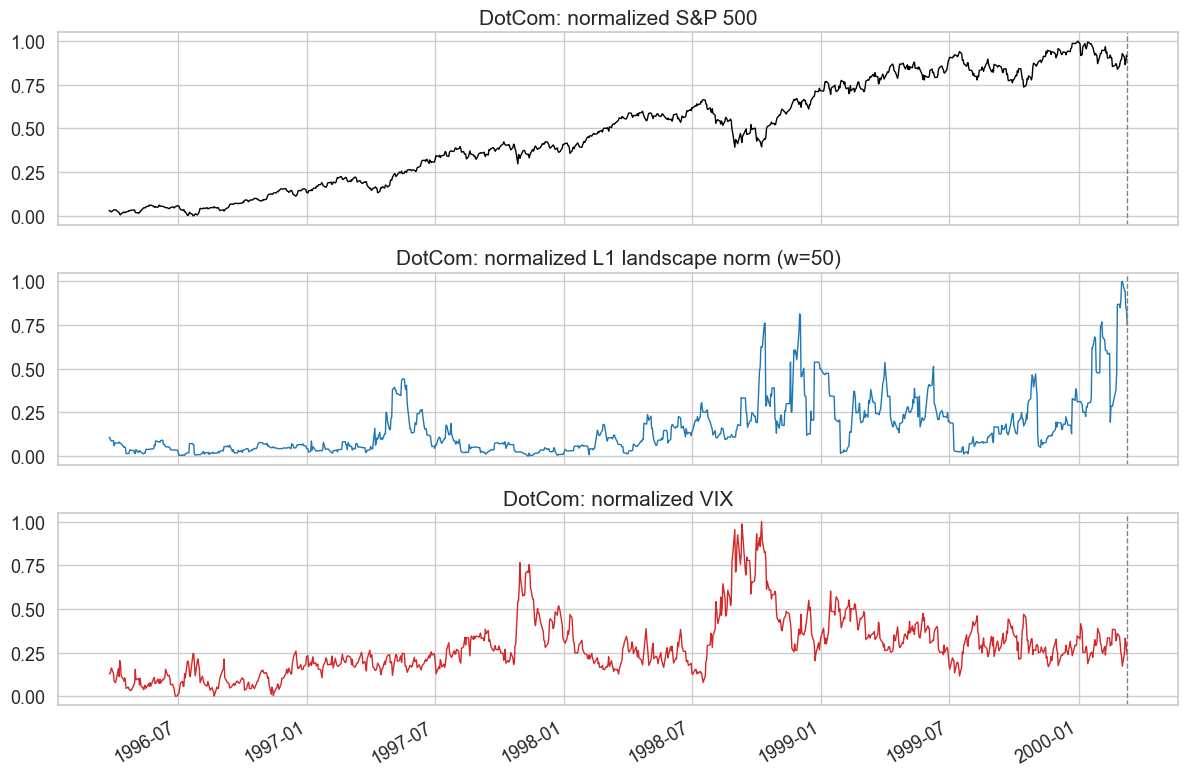
\includegraphics[width=0.49\textwidth]{figures/figure_cell15_out0.png}
    \hfill
    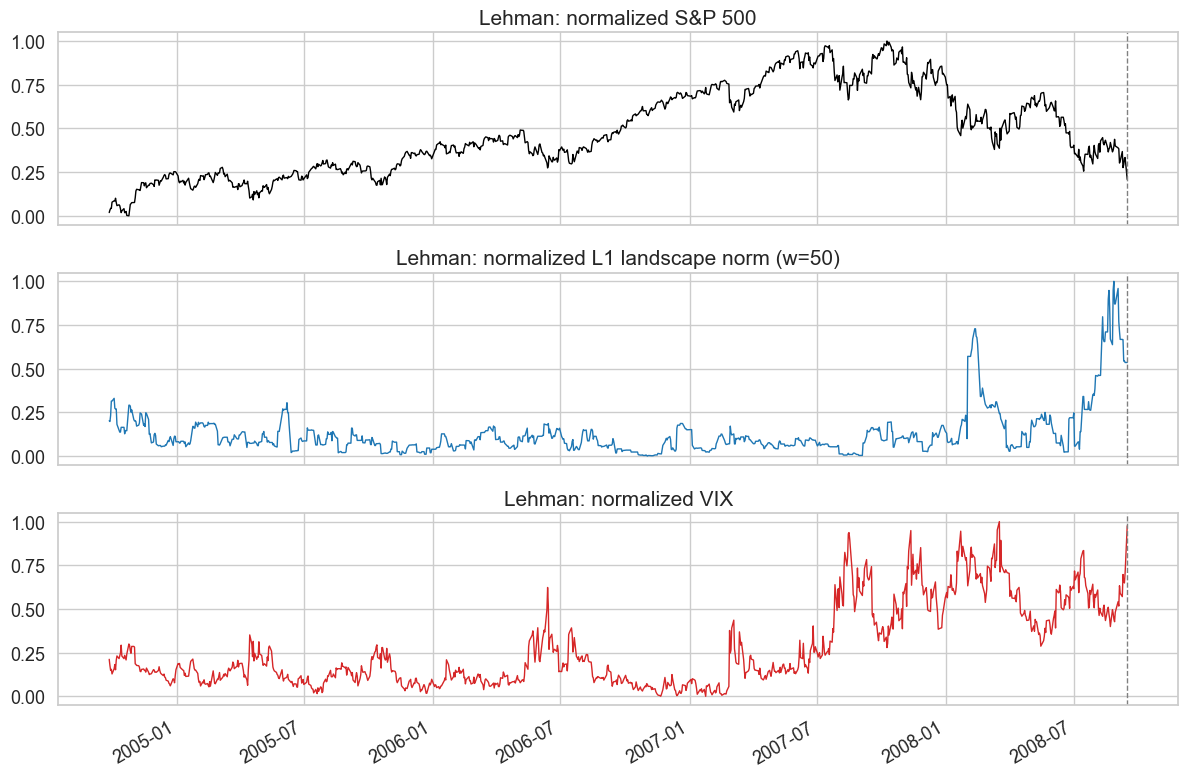
\includegraphics[width=0.49\textwidth]{figures/figure_cell15_out1.png}
    \caption{Normalized S\&P~500 trajectory, standardized $L^1$ ($w=50$), and normalized VIX centered on Dot-com (left) and Lehman (right).}
    \label{fig:rep_events}
\end{figure}

\begin{table}[htbp]
    \centering
    \begin{tabular}{lcc}
    \toprule
    Event & Variance trend ($\tau$, $p$) & Low-frequency PSD trend ($\tau$, $p$) \\
    \midrule
    Dot-com & $-0.223$, $1.44\times10^{-7}$ & $-0.602$, $1.42\times10^{-45}$ \\
    Lehman & $0.888$, $4.36\times10^{-97}$ & $0.691$, $1.40\times10^{-59}$ \\
    \bottomrule
    \end{tabular}
    \caption{Kendall-$\tau$ trend tests on variance and low-frequency power of landscape norms over 250 pre-anchor sessions.}
    \label{tab:rep_trends}
\end{table}
\FloatBarrier

Table~\ref{tab:rep_trends} supports the graphical results. The Lehman period shows strong positive trends in both variance and low-frequency spectral power, consistent with increasing market stress before the crisis. The Dot-com results are statistically significant but much less consistent across diagnostics. 

Overall, the replication reaches a similar conclusion to the original paper. Persistence landscape $L^1$ norms appear capable of signaling some major market disruptions, especially the Lehman Brothers collapse, but the results are noticeably weaker for the Dot-com period. This suggests that the effectiveness of the topological signal is not uniform across crises and may depend on the structure of the specific event.

\section{Extension: COVID-19 period}
\label{sec:extension}

To test whether the framework generalized beyond the original sample period, I extended the Yahoo Finance data through 2020 while keeping the same implementation, rolling windows, and parameter choices. This provides an out-of-sample test of whether persistence landscape norms behave similarly during (and most importantly, prior to) the COVID-19 market crash.

Figure~\ref{fig:ext_postpaper} compares standardized $L^1$ and $L^2$ persistence landscape norms across the two rolling window sized after the original replication sample. Both exhibit a strong spike around after March of 2020, but not prior to it. Quite on the contrary, the elevated norms are prevalent for a strong time after the spike but do not exhibit a predictive behavior for the upcoming market behavior.

\FloatBarrier
\begin{figure}[htbp]
    \centering
    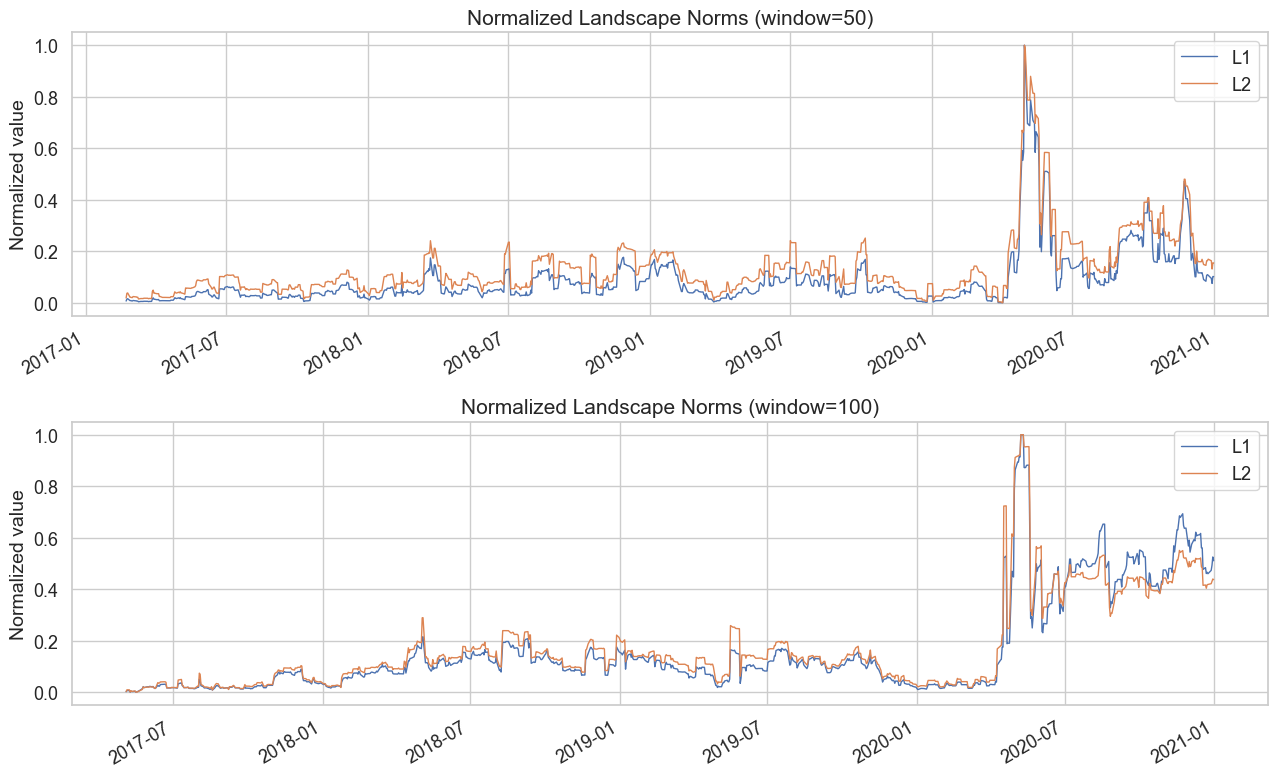
\includegraphics[width=\textwidth]{figures/extension_cell13_out0.png}
    \caption{Standardized $L^1$ landscape norms versus standardized VIX after the replicated sample window.}
    \label{fig:ext_postpaper}
\end{figure}

\begin{figure}[htbp]
    \centering
    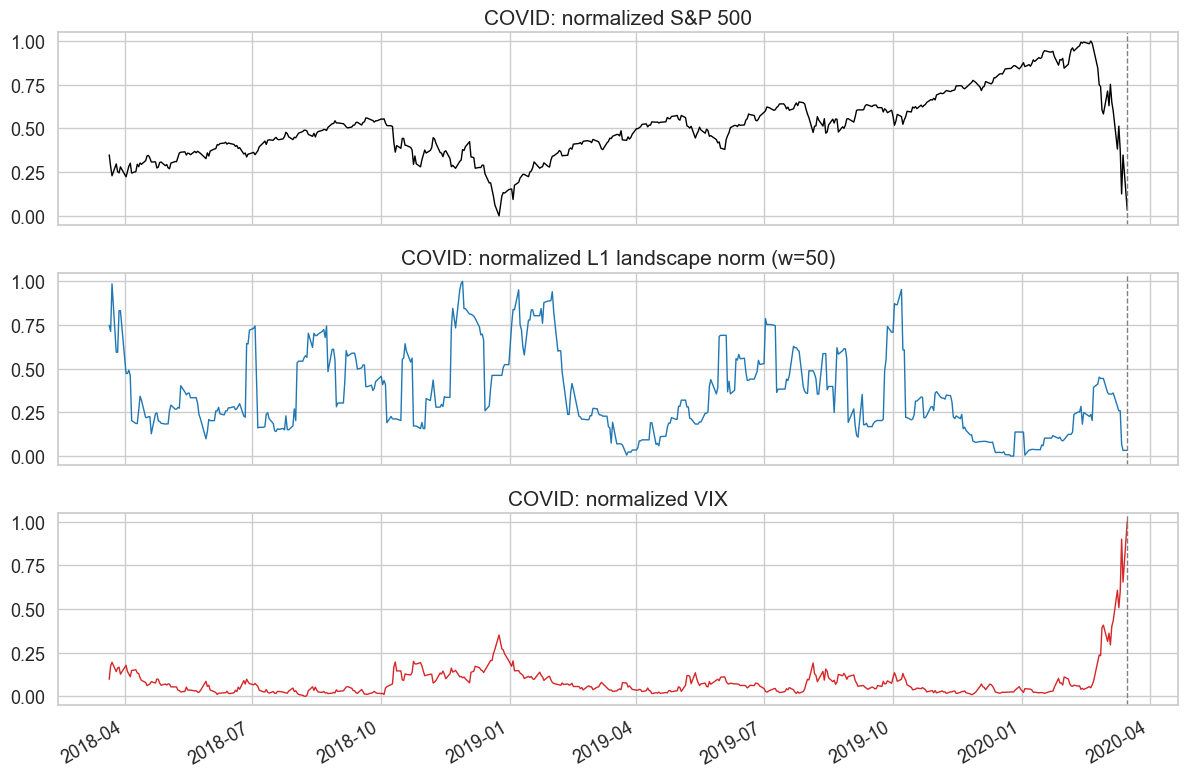
\includegraphics[width=\textwidth]{figures/extension_cell15_out0.png}
    \caption{COVID-focused window with normalized aggregate S\$P 500, persistence landscape $L^1$, and VIX.}
    \label{fig:ext_covid}
\end{figure}
\FloatBarrier

Figure~\ref{fig:ext_covid} focuses specifically on the COVID-19 crash. Unlike the Lehman event, the persistence landscape $L^1$ norms do not show a meaningful buildup before the market decline. In fact, the norms remain near historical lows leading into the February--March 2020 selloff, even as VIX rises sharply and equity markets collapse.

This result is important because it directly tests the robustness of the methodology outside the original sample. The COVID crash was one of the sharpest market disruptions in recent history, yet the persistence landscape norms provided little indication of the incoming stress. Under the unchanged setup, the topological signal was not only weak, but actually near all-time lows immediately before the crash.

One possible explanation is that the COVID shock developed too rapidly for rolling-window geometric summaries to capture structural changes ahead of time. Another possibility is that the persistence landscape framework is sensitive to the specific type of market crisis being studied. In either case, the extension results suggest that the predictive usefulness of the $L^1$ norms may be less stable than originally hoped.

\section{Conclusion and discussion}
\label{sec:discussion}

This project replicated the topological data analysis framework developed by Gidea and Katz and then extended the analysis through the COVID-19 market crash. The replication results broadly support the original paper's findings. Persistence landscape $L^1$ norms appear capable of identifying buildup patterns before some major financial crises, particularly the Lehman Brothers collapse. However, the results are much weaker for the Dot-com period, where the signals are less consistent across graphical and statistical measures.

The extension through 2020 provides a more challenging test of the framework. During the COVID-19 crash, the persistence landscape norms failed to show a meaningful early-warning signal and were actually near historical lows before the market decline. This contrasts sharply with the behavior observed during Lehman and suggests that the methodology may not generalize well across all crisis environments.

The main takeaway from this project is that studying the topology of financial markets is still an interesting and valuable research direction. Persistent homology provides a different way to analyze market structure by focusing on the geometry of joint returns instead of only volatility or correlations. The framework clearly captures meaningful structural changes during some periods of market stress.

At the same time, the results suggest that persistence landscape norms are probably not as robust or universal an indicator as the original paper may have implied. Their effectiveness appears highly dependent on the type of crisis, the timing of the shock, and the parameter choices used in the rolling-window construction. As a result, these topological indicators are better interpreted as exploratory tools that complement traditional financial measures rather than reliable stand-alone forecasting signals.


\newpage
\section*{Appendix}

Figure~\ref{fig:rep_data} confirms adjusted-close levels and daily log-return alignment among the replication inputs prior to applying persistent homology.

\begin{figure}[htbp]
    \centering
    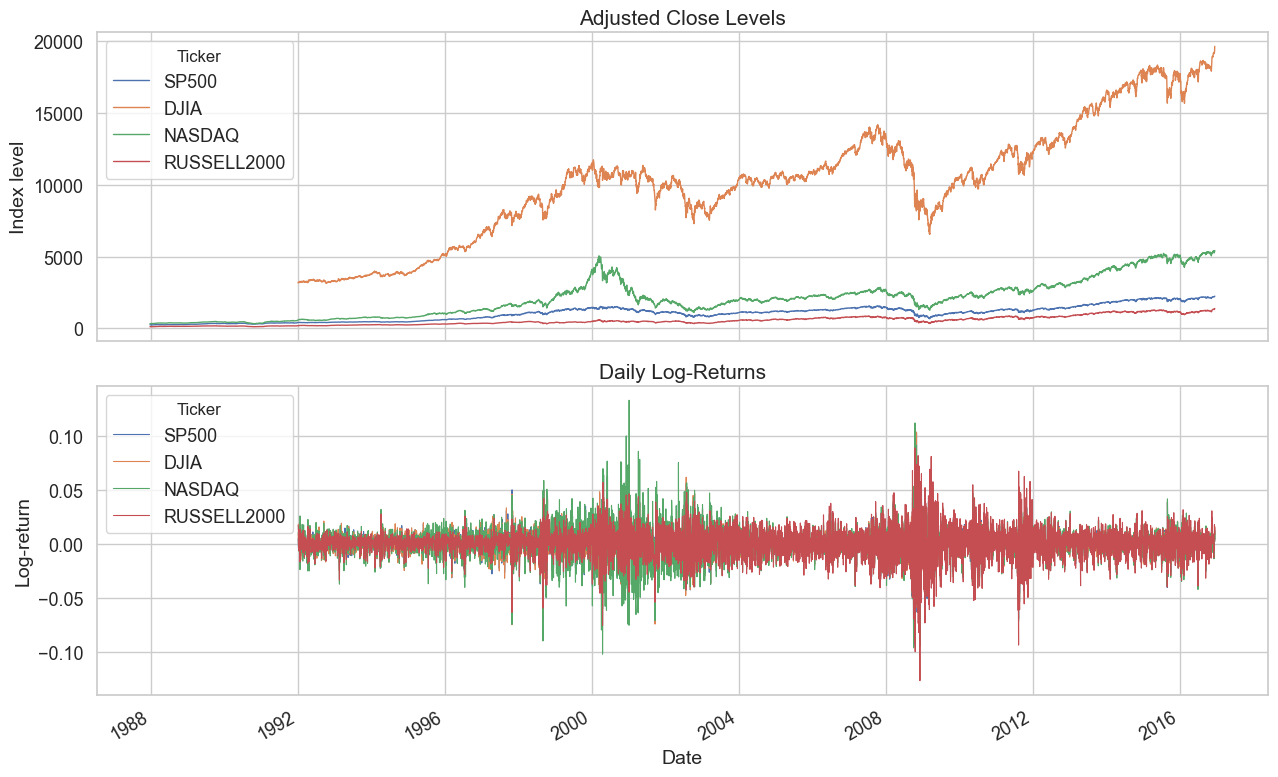
\includegraphics[width=\textwidth]{figures/figure_cell7_out0.png}
    \caption{Adjusted-close levels and aligned daily log-returns for instruments entering the topological pipeline.}
    \label{fig:rep_data}
\end{figure}

\end{document}